\documentclass{article}

\usepackage{amsmath}
\usepackage{fancyhdr}
\usepackage{graphicx}
\graphicspath{{}}

%% some colours
\usepackage{color}
\definecolor{deepblue}{rgb}{0,0,0.5}
\definecolor{deepred}{rgb}{0.6,0,0}
\definecolor{deepgreen}{rgb}{0,0.5,0}
\definecolor{backcolour}{rgb}{0.95,0.95,0.92}


%%%%%%%%%%%%%% CODE STUFF %%%%%%%%%%%%%%
%%%%%%%%%%%%%%%%%%%%%%%%%%%%%%%%%%%%%%%%
\usepackage{listings} % for code display
% setting code style
\newcommand\pythonstyle{\lstset{
language=Python,
backgroundcolor=\color{backcolour},
otherkeywords={self},             % Add keywords here
keywordstyle=\color{deepblue},
emphstyle=\color{deepred},    % Custom highlighting style
stringstyle=\color{deepgreen},
frame=tb,                         % Any extra options here
showstringspaces=false            % 
}}

% Python environment
\lstnewenvironment{python}[1][]{
    \pythonstyle
    \lstset{#1}
}{}

% Python for external files
\newcommand\pythonexternal[2][]{{
    \pythonstyle
    \lstinputlisting[#1]{#2}
}}

% Python for inline
\newcommand\pythoninline[1]{{\pythonstyle\lstinline!#1!}}

%%%%%%%%%%%%%%%%%%%%%%%%%%%%%%%%%%%%%%%%

\title{BPP Exercise 2 - The Very Basics}
\author{A. Hain, M. Nipshagen}
\date{16.04.2018, 8:00}

\makeatletter
\let\thetitle\@title
\let\theauthor\@author
\let\thedate\@date
\makeatother

\pagestyle{fancy}
\fancyhf{}
\fancyhead[L]{\thetitle}
\fancyhead[C]{}
\fancyhead[R]{\theauthor}
\renewcommand{\headrulewidth}{0.4pt} %obere Trennlinie
\fancyfoot[L]{Due: \thedate}
\fancyfoot[R]{\thepage} %Seitennummer
\renewcommand{\footrulewidth}{0.4pt}

% include solutions
\newcommand\sol[1]{#1}
% do not include solutions
% \newcommand\sol[1]{       }

\begin{document}

The deadline for this exercise sheet is \textbf{Monday, \thedate.}
%
%\section*{Introductory Words}
%In case we have some information that doesn't directly concern the current exercises.
%
\section{Variable Types}
Assume you're enrolled in a Psychology class.
Your final grade is dependent on your performance in homework, a midterm exam and an experiment as a final project.\\
\textit{Note:} Save your answers for this task in a simple text file.

\subsection{}
You just wrote the midterm and after correcting, your professor thinks it might be handy
to have the exam results for each student digitally accessible. Which variable types would you use
for variables to save the following things in? Explain your answers.
\begin{enumerate}
\item the student's name
\item the student's matriculation number
\item the student's exam grade
\item if the student passed the exam or not
\end{enumerate}

\sol{\begin{enumerate}
    \item student's name: String
    \item matriculation number: Int or String
    \item Exam Grade: Float
    \item Passed: Boolean
\end{enumerate}}

\subsection{}
Fast foward some time, you need to conduct the experiment. In the experiment you
present subjects with a short stimulus and measure their score based on reaction.
Each subject in the end has 4 scores, and you calculate their overall performance
with the following formula $$ \dfrac{4*Score1 + Score2 + 0.5*Score3 + \sqrt{Score4}}{2\pi} $$
\emph{Note:} Totally arbitrary forumla with probably no real world use.\\
You can approximate \(\pi \) with 3.14 or you can use the following to get pi in python:
\begin{python}
    import math.pi

    print(pi)
\end{python}

Write a function that calculates and returns the overall performance of a subject when you pass it the five scores.

\section{Some Calculations [insert better task name maybe]}
In this task, you will have to write two small Python programs. Please save each
of them in a separate file.

\subsection{-}
After you completed your Psychology class, your professor now wants to determine your final grade.
It is composed of your homework grade by 20\%, your midterm grade by 30\% and your final
project grade by 50\%.\\
Write a Python script which will calculate the final grade out of those three grades
and print the result. Try to use suitable names for your variables and test your program with
a few different values.

\subsection{The cake is no lie}
After passing the class, you want to treat yourself by baking
a chocolate cake. You find a nice recipe for the dough online. The quantities of
the ingredients are perfect to make one cake in a circular cake mould with a diameter
of 28cm and a height of 8cm. However, you only have a cake mould with a diameter of 24cm and a height of 6.5cm.\\
What is the factor if you only have a cake mould with a 20cm diameter/6cm height or 18cm diameter/6cm height?\\
Write a script that contains a function to determine by which factor you need to multiply the cake ingredients to make the perfect amount of dough for your smaller cake moulds and prints the result.\\

\begin{center}
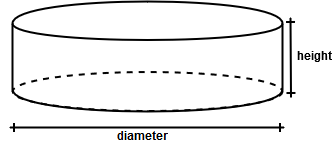
\includegraphics[scale=0.6]{Ex_2_Cake}
\end{center}

\end{document}
